Transimpedance Amplifiers (TIAs) are current to voltage converters generally implemented using one operational amplifier, as shown in \autoref{fig:TIA_basic} \cite{horowitz1989art}. A current coming from the negative input of the op-amp is amplified and converted to a voltage signal by a feedback resistor $R_f$, while the positive input of the op-amp is connected to the reference. TIAs are negative gains amplifiers similar to inverting amplifiers configuration. For DC applications, their transimpedance follows the equation: 
\begin{equation}
\label{eq:TIA_simple}
G(\omega=0)=\frac{V_{out}}{I_{in}} = -R_f
\end{equation}
Large values of feedback resistors are generally chosen in TIAs since the transimpedance increases linearly with $R_f$, while the output voltage noise, when only considering  the Johnson-Nyquist noise due to the thermal agitation of charge carriers, increase proportionally to its root mean squared value \cite{horowitz1989art}. This leads to an input-refered noise current proportional to the inversed root mean square of $R_f$: 
\begin{equation}
\sqrt{i_{n,in}^2}=\sqrt{\frac{4 k_B T \Delta f}{R_f}}
\end{equation}
However, choosing large values of $R_f$ induce considerable output offset voltage and large output voltage swing \cite{horowitz1989art}. It is thus recommended to use op-amps based on Field-Effect Transistors (FET) that present a low input offset voltage, and op-amps featuring a high gain-bandwidth product when higher excitation frequencies are used \cite{horowitz1989art}. \par
\begin{figure}[h]
    \centering
    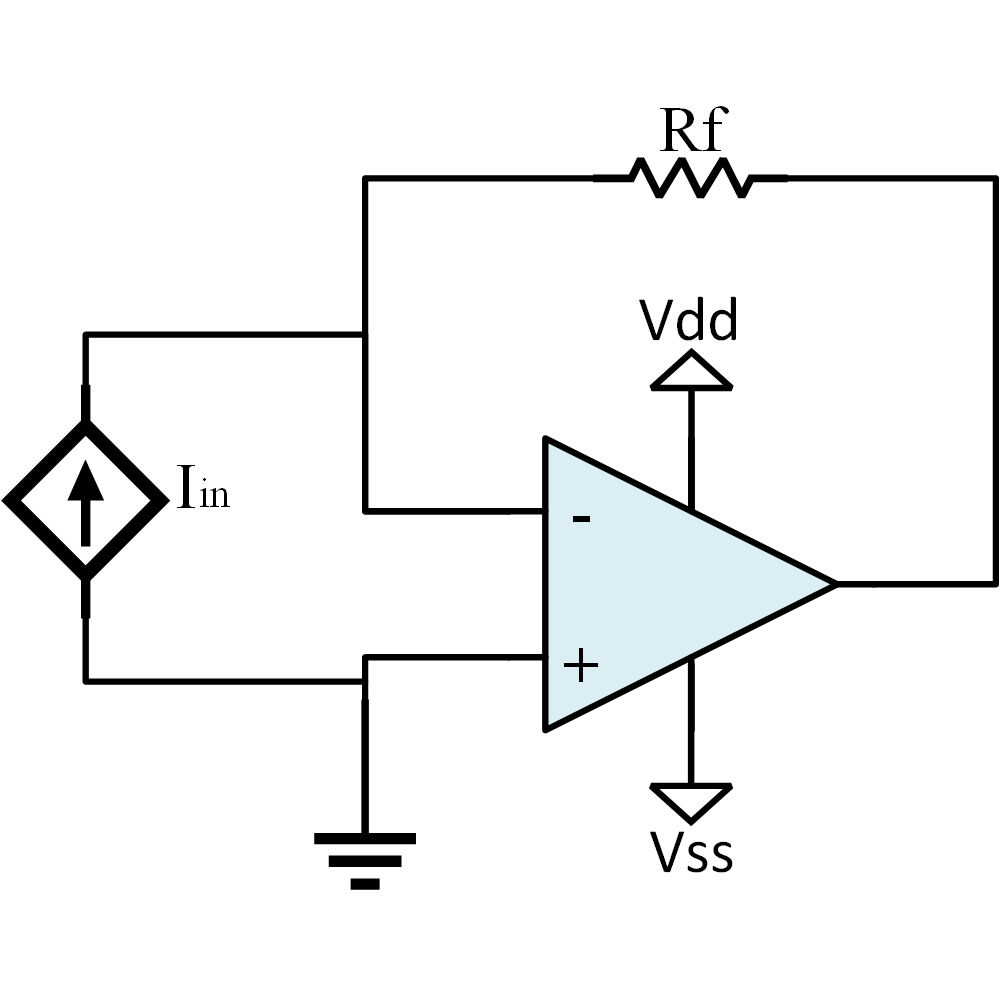
\includegraphics[width=0.5\textwidth]{TIA_basic}
    \caption{A basic discrete TIA made from one op-amp and one resistor.}
    \label{fig:TIA_basic}
\end{figure}
A case must be presented concerning the stability of TIAs. An input capacitance $C_i$, often caused by parasitics or by the sensor itself, introduces a pole in the transfer function which induces oscillation at a specific frequency $f_i$ \cite{horowitz1989art}. This is the case since a negative phase-shift is created by the pole, which, when combined with the $180^{\circ}$ phase inversion of the TIA, can induce a full 360 $^{\circ}$ phase-shift, effectively producing a positive feedback loop. If this positive feedback is obtained for a unity or larger op-amp open-loop gain $A_{OL}$, unrestricted oscillations will be generated \cite{horowitz1989art}. This can be better shown mathematically, where the output voltage for an uncompensated TIA is described the same way as in Equation XXX, but with an added pole:
\begin{equation}
V_{out}=I_{in} \frac{-R_f}{1+\frac{1+ R_f C_i s}{A_{OL}}}
\end{equation}
A feedback capacitor $C_f$ can be introduced in parallel with $R_f$ to compensate for the added pole, as shown in \autoref{fig:TIA_compensated}. This leads to a phase cancellation of the pole, which, for an adequate choice of $C_f$, negates the positive feedback loop. The new transfer function is described here: 
\begin{equation}
\label{eq:TIA_full}
V_{out}=I_{in} \frac{-R_f}{1+\frac{1+ R_f (C_i + C_f) s}{A_{OL} (1+ R_f C_f s)}}
\end{equation}
There is no proper method to calculate the compensation capacitor $C_f$. Using a large capacitor will result in a decreased amplifier bandwidth, while a small capacitor may be unable to prevent oscillations\cite{horowitz1989art}. A sufficient phase margin should be considered to prevent unwanted anomalies, which justifies using an iterative approach. Another shortcoming of this approach is that the feedback capacitor value is oftentimes really small when using large resistor values. This effectively creates a compromise when designing TIAs between capacitor choice, thermal noise, offset voltage, bandwidth, and stability. 
\begin{figure}[h]
    \centering
    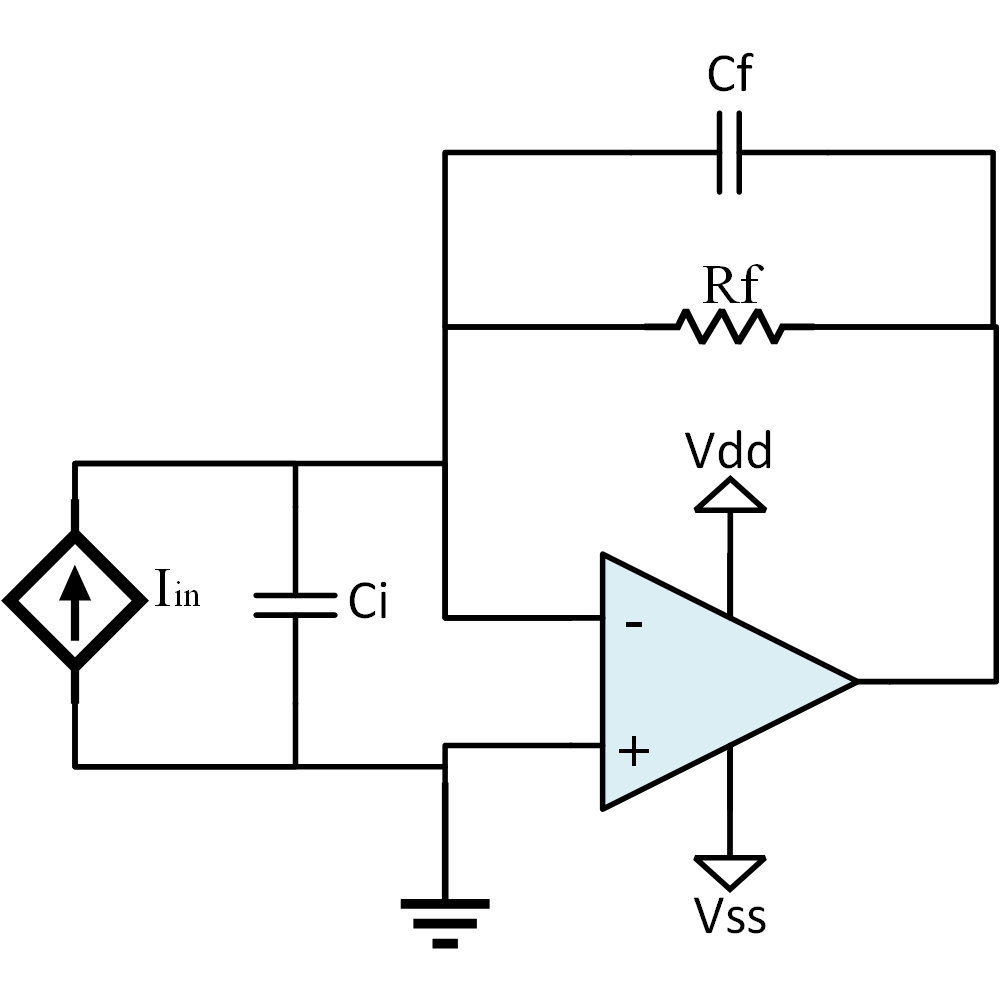
\includegraphics[width=0.5\textwidth]{TIA_compensated}
    \caption{Typical application circuit of a compensated discrete TIA. The pole introduced by the input capacitance $C_i$ is compensated by the feedback capacitor $C_f$}
    \label{fig:TIA_compensated}
\end{figure}